\subsection{Análise Estatística e Validação por Simulação de Monte Carlo do Teste A/B}
\label{subsec:analise_teste_ab_monte_carlo}

Nesta seção, é apresentada a análise estatística dos dados gerados pelo experimento computacional executado em ambiente $R$. O estudo consiste em um Teste A/B projetado para avaliar o impacto da alteração cromática de um botão de ação de uma interface digital sobre a taxa de conversão de usuários. O experimento foi conduzido sob condições controladas, dividindo-se uniformemente uma amostra total em dois grupos de tamanhos idênticos ($A_n = B_n = 2500$): o Grupo A (Controle), que utilizou a interface padrão com o botão na cor Azul, e o Grupo B (Tratamento), submetido à nova interface com o botão na cor Verde.

\subsubsection{Resultados Amostrais Observados}

A execução do experimento gerou realizações empíricas a partir de processos estocásticos binomiais independentes. Os dados agregados revelaram as seguintes taxas de conversão amostrais:
\begin{itemize}
	\item Grupo A: Taxa de conversão observada de $ P(A) = 9,56\%$, correspondendo a $239$ conversões confirmadas.
	\item Grupo B: Taxa de conversão observada de $ P(B) = 13,56\%$, correspondendo a $339$ conversões confirmadas.
\end{itemize}

A diferença bruta observada entre o grupo de tratamento e o grupo de controle foi de $ P(B) -  P(A) = 4,00\%$. A distribuição visual dessa discrepância inicial entre os dois grupos pode ser observada no gráfico de barras apresentado na Figura~\ref{fig:taxas_conversao_obs}.

\begin{figure}[ht]
	\centering

	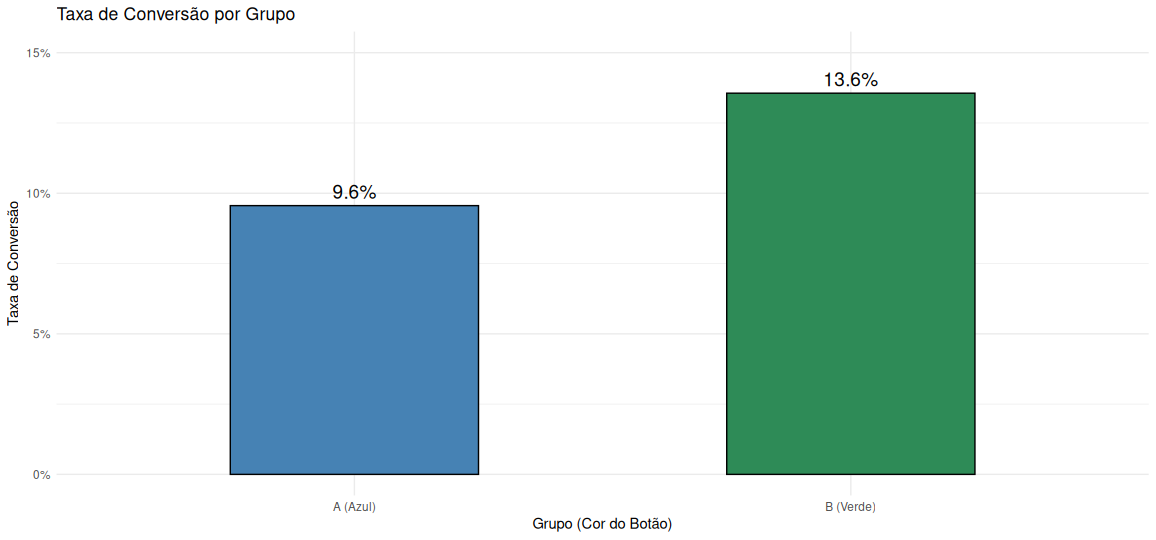
\includegraphics[width=0.65\textwidth]{secoes/07_atividade_integradora/atv_3/imagens/taxa_de_conversao_por_grupo.png}
	\caption{Comparação das taxas de conversão observadas entre o Grupo A e o Grupo B.}
	\label{fig:taxas_conversao_obs}
\end{figure}

\subsubsection{Modelagem Frequentista e Teste de Hipóteses}

Para determinar se o incremento de $4,00\%$ na taxa de conversão a favor do botão Verde possui significância estatística ou se decorre meramente de flutuações aleatórias do processo de amostragem, aplicou-se o teste Z de igualdade de duas proporções assintótico. O teste foi configurado de forma bicaudal, sem a correção de continuidade de Yates. As hipóteses estatísticas formalizadas são:

\begin{align*}
	H_0: &P(B) - P(A) = 0 \quad \text{(A cor do botão não exerce efeito sobre a taxa de conversão)} \\
	H_1: &P(B) - P(A) \neq 0 \quad \text{(A alteração cromática afeta significativamente a taxa de conversão)}
\end{align*}

Os resultados numéricos computados a partir da distribuição qui-quadrado ($\chi^2$) associada ao teste Z são descritos a seguir:
\begin{itemize}
	\item \textbf{Estatística de Teste ($\chi^2$):} $19,562$ (com grau de liberdade $df = 1$).
	\item \textbf{$p$-valor:} $9,736 \times 10^{-6}$ (ou $0,000009736$).
	\item \textbf{Intervalo de Confiança de 95\%:} $[-0,05769; -0,02231]$ para a diferença $P(A) - P(B)$, o que equivale a um ganho líquido estatisticamente estimado entre $2,23\%$ e $5,77\%$ a favor do Grupo B.
\end{itemize}

Considerando o nível de significância ($\alpha = 0,05$), a hipótese nula $H_0$ é estritamente rejeitada, dado que o $p$-valor obtido é substancialmente inferior ao limiar ($p < 0,05$). Infere-se que a mudança de cor para Verde aumenta a taxa de conversão.

\subsubsection{Validação Empírica via Simulação de Monte Carlo}

Com o intuito de verificar o modelo teórico paramétrico frente a uma abordagem empírica, estruturou-se uma Simulação de Monte Carlo fundamentada em $10.000$ experimentos sintéticos independentes sob as premissas estritas de $H_0$. Para tal fim, parametrizou-se uma taxa de conversão base e comum de $P(H0) = 10,00\%$ para ambas as distribuições.

De acordo com o referencial teórico assintótico, a variância amostral da diferença entre duas proporções independentes sob a hipótese nula é governada pelo erro padrão teórico ($\sigma_{\text{teórico}}$), calculado por:

\begin{equation}
	\sigma_{\text{teórico}} = \sqrt{P(H0) \cdot (1 - P(H0)) \cdot \left( \frac{1}{n_A} + \frac{1}{n_B} \right)} 
\end{equation}

Substituindo os parâmetros do estudo ($P(H0) = 0,10$ e $A_n = B_n = 2500$), obtém-se o desvio padrão teórico da distribuição amostral nula:

\begin{equation}
	\sigma_{\text{teórico}} = \sqrt{0,10 \cdot 0,90 \cdot \left( \frac{1}{2500} + \frac{1}{2500} \right)} = \sqrt{0,000072} \approx 0,008485 \quad (0,85\%)
\end{equation}

A Figura~\ref{fig:teoria_vs_simulacao} apresenta o confronto direto entre a distribuição de frequências obtida empiricamente pelas $10.000$ simulações e a curva de densidade normal teórica idealizada.

\begin{figure}[ht]
	\centering
	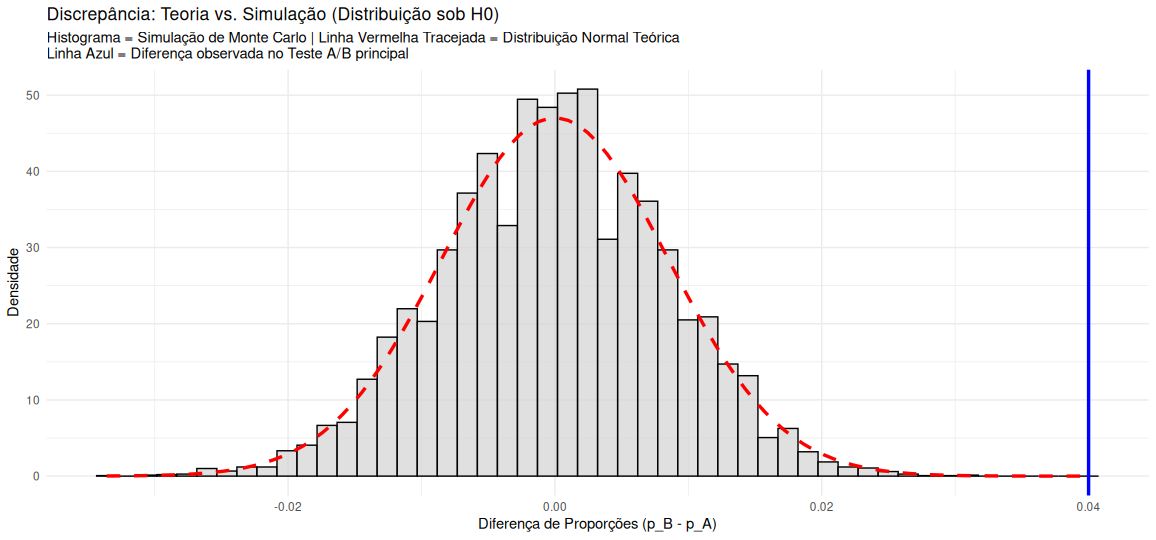
\includegraphics[width=0.85\textwidth]{secoes/07_atividade_integradora/atv_3/imagens/teoria_vs_simulacao.png}
	\caption{Distribuição nula da diferença de proporções: Histograma empírico da Simulação de Monte Carlo vs. Curva Normal Teórica (linha tracejada vermelha) e o valor real observado (linha azul).}
	\label{fig:teoria_vs_simulacao}
\end{figure}

A convergência dos dados expressa na Figura~\ref{fig:teoria_vs_simulacao} permite extrair duas conclusões fundamentais para a validação metodológica:
\begin{enumerate}
	\item \textbf{Aderência do Modelo Assintótico:} O histograma gerado via Monte Carlo replica  a curva Gaussiana teórica de comportamento paramétrico. Esse comportamento chancela a aplicação do Teste Z assintótico, assegurando que o tamanho da amostra coletada ($n = 2500$ por grupo) é perfeitamente adequado para mitigar distorções de amostragem.
	\item \textbf{Visualização do Limiar Crítico:} A linha vertical azul representa o resultado obtido no teste real original ($P(B) - P(A) = 0,04$). Graficamente, observa-se que a diferença observada de $4,00\%$ localiza-se no extremo da cauda direita da curva de probabilidade. Calculando o escore padronizado, verifica-se que este ponto situa-se a $Z = \frac{0,04}{0,008485} \approx 4,71$ desvios padrões de distância em relação à média zero esperada sob $H_0$. Tal distanciamento corrobora visualmente o $p$-valor e confirma que o comportamento observado do botão Verde é estatisticamente superior.
\end{enumerate}


\subsubsection{Implementação Computacional}

\begin{lstlisting}[language=R, caption={}, label=]
library(ggplot2)
library(dplyr)
set.seed(42)

# Tamanho da amostra por grupo (visitantes)
n_A <- 2500 
n_B <- 2500

# Vamos assumir que o botão Verde (B) é de fato melhor
p_A_verdadeiro <- 0.10
p_B_verdadeiro <- 0.13 

# Simulando o número de conversões usando a distribuição Binomial
conv_A <- rbinom(n = 1, size = n_A, prob = p_A_verdadeiro)
conv_B <- rbinom(n = 1, size = n_B, prob = p_B_verdadeiro)

# Taxas observadas na amostra
p_A_obs <- conv_A / n_A
p_B_obs <- conv_B / n_B

cat("--- Resultados do Experimento Observado ---\n")
cat("Taxa de Conversão Grupo A (Controle):", round(p_A_obs * 100, 2), "%\n")
cat("Taxa de Conversão Grupo B (Tratamento):", round(p_B_obs * 100, 2), "%\n\n")

# Aplicando o teste Z de proporções
teste_ab <- prop.test(x = c(conv_A, conv_B), 
n = c(n_A, n_B), 
alternative = "two.sided", 
correct = FALSE)

print(teste_ab)


p_valor <- teste_ab$p.value
if(p_valor < 0.05) {
	cat("\nConclusão: Rejeitamos H0 (p-valor =", p_valor, "). Há evidência estatística de que o botão Verde converte mais.\n")
} else {
	cat("\nConclusão: Falhamos em rejeitar H0 (p-valor =", p_valor, "). Não há evidência suficiente de diferença.\n")
}


n_simulacoes <- 10000
p_h0 <- 0.10

# Simulação de Monte Carlo vetorizada para velocidade
sim_A <- rbinom(n_simulacoes, n_A, p_h0) / n_A
sim_B <- rbinom(n_simulacoes, n_B, p_h0) / n_B
diferencas_simuladas <- sim_B - sim_A

# Parâmetros teóricos da Normal sob H0
erro_padrao_teorico <- sqrt(p_h0 * (1 - p_h0) * (1/n_A + 1/n_B))


df_simulacao <- data.frame(Diferenca = diferencas_simuladas)

# Gráfico 1: Taxas de Conversão Observadas
df_barras <- data.frame(
Grupo = c("A (Azul)", "B (Verde)"),
Taxa = c(p_A_obs, p_B_obs)
)

g1 <- ggplot(df_barras, aes(x = Grupo, y = Taxa, fill = Grupo)) +
geom_bar(stat = "identity", width = 0.5, color = "black") +
geom_text(aes(label = scales::percent(Taxa, accuracy = 0.1)), vjust = -0.5, size = 5) +
scale_fill_manual(values = c("steelblue", "seagreen")) +
scale_y_continuous(labels = scales::percent, limits = c(0, 0.15)) +
labs(title = "Taxa de Conversão por Grupo",
y = "Taxa de Conversão", x = "Grupo (Cor do Botão)") +
theme_minimal() +
theme(legend.position = "none")

print(g1)

# Gráfico 2: Teoria vs Simulação (Distribuição Nula)
g2 <- ggplot(df_simulacao, aes(x = Diferenca)) +
geom_histogram(aes(y = ..density..), bins = 50, fill = "lightgray", color = "black", alpha = 0.7) +

stat_function(fun = dnorm, args = list(mean = 0, sd = erro_padrao_teorico), 
color = "red", size = 1.2, linetype = "dashed") +

geom_vline(xintercept = (p_B_obs - p_A_obs), color = "blue", size = 1.2) +
labs(title = "Discrepância: Teoria vs. Simulação (Distribuição sob H0)",
subtitle = "Histograma = Simulação de Monte Carlo | Linha Vermelha Tracejada = Distribuição Normal Teórica\nLinha Azul = Diferença observada no Teste A/B principal",
x = "Diferença de Proporções (p_B - p_A)",
y = "Densidade") +
theme_minimal()

print(g2)


\end{lstlisting}


